\chapter{Computational methods}
\label{ch:Computational methods}
In this section a number of computational methods that can be used for conceptual structural design are introduced. 

\section{Form Finding}
Physical models or numerical simulations can be used for form finding, where the aim is to find the form for a structure under load where static equilibrium is satisfied. The static equilibrium corresponds to a structure that can support the applied load using only compression or tension, thus a very efficient structure. For physical models a hanging chain or cloth can be used the find the static equilibrium.

A number of different form finding methods exists, and they can be divided into three major categories \cite{Veenendaal2012a}: 

\begin{itemize} 
\item Stiffness matrix methods - which are based on elastic and geometric stiffness matrices. These methods have adapted methods structural analysis for form finding.
\item Geometric stiffness methods - these methods are material independent. The first such example is the force density method \cite{Schek1974} which makes use of the ratio of force to length. Several other methods have been developed which extends on this work.
\item Dynamic equilibrium methods - these methods find the steady-state equilibrium through use of dynamics. One such method is dynamic relaxation \cite{Day1965} which is explained in further detail in Section \ref{sec:dr}.
\end{itemize} 

\begin{figure}
  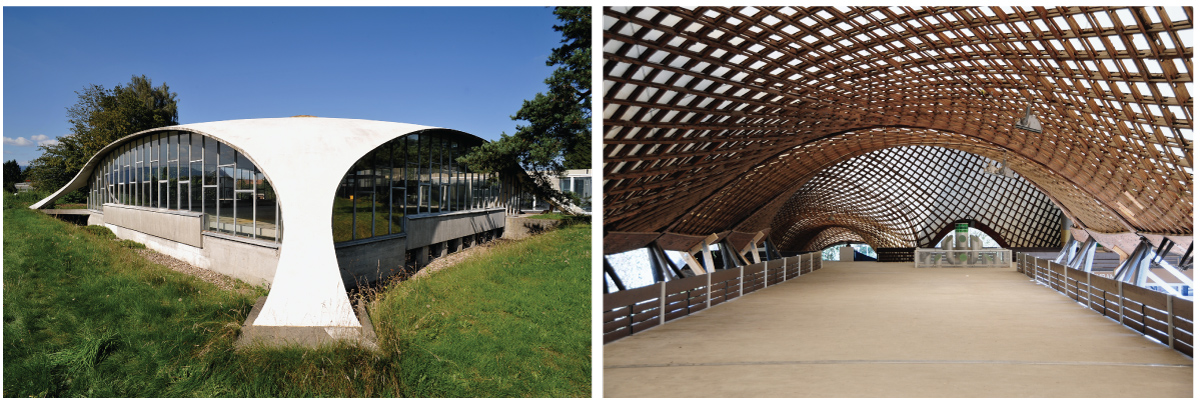
\includegraphics[width=380pt]{graphics/formfinding-ex.jpg}
  \caption{Example of formfound structures. Left: Concrete dome by Heinz Isler, © Chriusha, Wikimedia Commons; Right: Multihalle in Mannheim by Frei Otto }
  \label{fig:Stevin}
\end{figure}

\subsection{Dynamic relaxation}
\label{sec:dr}
Dynamic relaxation is a method to solve a set of non-linear equations. The method computes the movement of a structure over time to find static equilibrium between the internal and external forces \cite{Day1965, barnes1988form}. 

In each time step,  $\Delta t$, for all elements are computed from the nodal displacements u. A residual, R, can be computed by using 

\begin{equation*}
  R = f_{ext} - F_{int} 
\end{equation*}

Where $f_{ext}$ is the external forces acting on the structure. By using Newton’s second law the acceleration (time derivative of the velocity) can be computed as follows (at the node i, in the x-direction, at the time t)

\begin{equation*}
  R^t_{ix} = M_i  \cdot \dot{v}^t_{ix}
\end{equation*}

 is a lumped, fictitious mass at node i. To enforce boundary conditions, the residual is set to zero for the corresponding degrees of freedom. With the time step known the velocity of node i in the x-direction can be computed using finite difference method

\begin{equation*}
  v^{t+\Delta t}_{ix} = v^{t-\Delta t}_{ix} + \frac{\Delta t}{M_i} \cdot R^t_{ix}
\end{equation*}

With the velocity known the updated geometry can now be updated by using

\begin{equation*}
  x^{t+\Delta t}_{ix} = x^t_i + \Delta t \cdot v_{ix}^{t-\Delta t / 2}
\end{equation*}

As the geometry is updated, an iteration is complete and the computations start over, by again, computing the residual. The geometry is modified in each iteration until equilibrium between external and internal forces has been reached. Viscous or kinetic damping is often used in order for the method to converge \cite{barnes1988form}.

A recent development is a formulation that combines CAD-geometry and dynamic relaxation \cite{Alic2015} for form-finding.

\section{Optimization methods}
Michell was a pioneer in the field of structural optimization \cite{Michell1904} when he in 1904 published his results with minimum-weight Michell trusses. These trusses are still used today as benchmarks for topology optimization with framed trusses \cite{Clune2013}. 

Structural optimization is a numerical method to find the best solution for a mathematically formulated objective function that is subject to a set of constraints. The following variables are always present in structural optimization \cite{christensen2008introduction}:

\begin{itemize} 
\item \textit{Objective function (f) }- A function to classify designs from a quantifiable objective, the function returns a numerical value that represents how good the design is out of one or more criteria. Usually a small number is better then a large, i.e. a minimization problem. Frequently f measures weight, maximum displacements, strain energy or cost.
\item \textit{Design variable (x)} – A vector that describes the design with numerical values, it often represents a topology, nodal positions, cross sectional area or material.
\item \textit{State variable (y)} – For a given design with the design vector x, y represents the response of the structure i.e. how well the structure is performing from the evaluated criterion.
\end{itemize} 

The optimization problem can now be described as follows \cite{christensen2008introduction} :

\begin{equation}
SO=\begin{cases}
    \textrm{minimize } f(x,y) \textrm{ with resepct to } x \textrm{ and } y \\
    {\textrm{subject to} \begin{cases}
        \textrm{behavioral constraints on } y\\
        \textrm{design constraints on } x\\
	\textrm{equilibrium constraints} \\
    \end{cases}}
      \end{cases}
    \end{equation} 


 A number of different numerical methods exist to perform the optimization, and the best method depends on the solution space for the problem. A problem can also have multiple objective functions, so called multi-objective optimization. Which can be formulated as follows:

\begin{equation*}
minimize(f_1(x,y),f_2(x,y), \dotsc, f_n(x,y))
\end{equation*}

This is not a standard optimization problem as the objective functions are optimized for the same design variables. Instead a so-called Pareto optimality is sought, where there is no other design that satisfies all the objectives better \cite{christensen2008introduction}. If no single Pareto optimal point exists instead a Pareto front can be found in the objective space, where the objective space is a space with the different objectives on the axis. The objects can for example be, structural efficiency, operational energy consumption, sunlight etc.

\subsection{Gradient based methods}
\begin{figure}
  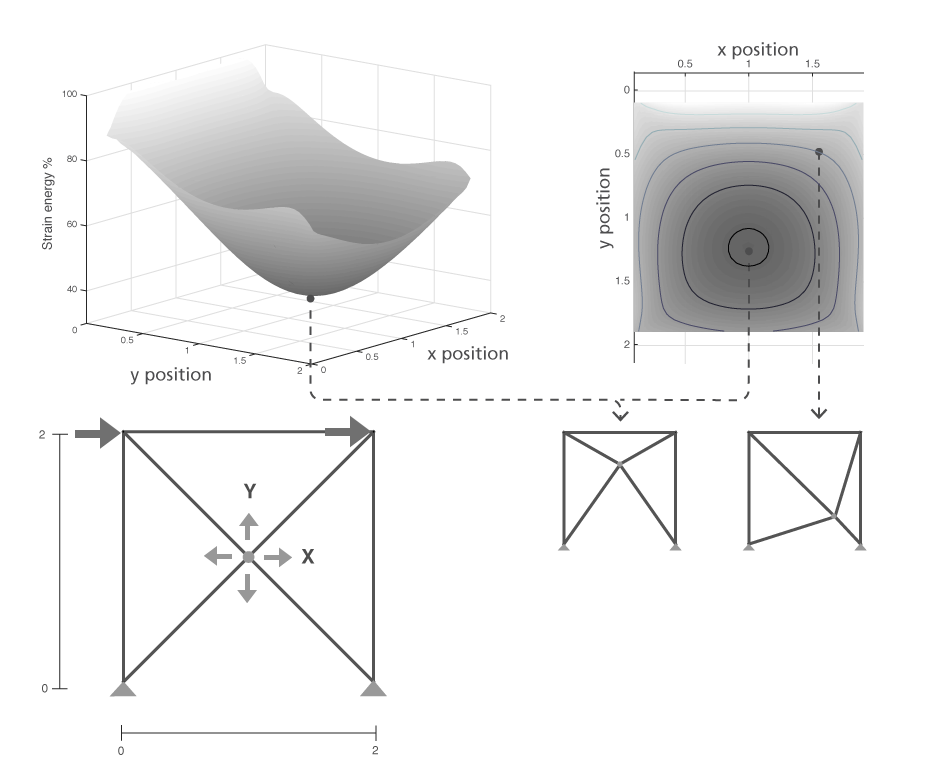
\includegraphics[width=310pt]{graphics/designspace.png}
  \caption{Design space for a shape optimization problem}
  \label{fig:designspace}
\end{figure}

Gradient-based methods make use of the first, and some the second, derivative to iteratively converge towards a solution. These types of methods are fast, consistent and the result is repeatable (no randomness). However, the solution space of the objective function needs to be convex (such as the design space in Figure \ref{fig:designspace}), continuous and at least once differentiable. The problem with using this type of methods for engineering and design, is that the problems are often so-called messy problems \cite{schlaich2006challenges}, that is non-convex solution spaces that contain multiple local optima. Examples of gradient-based methods are steepest descent and Newton-Rhapson \cite{christensen2008introduction}. 

\subsection{Evolutionary algorithms}
Evolutionary algorithms are a collection of generic population-based heuristic optimization algorithms \cite{Bangert2012}. The algorithms are inspired by biological evolution, survival of the fittest and natural selection. The solvers introduce randomness to search the solution space, which improves the algorithms ability to find the global optima.

One of the most well-known and used algorithms in this category is named genetic algorithm \cite{Goldberg1989}, it is inspired by the biological evolution. The benefits of this algorithm are that it is very robust and always returns a solution and the objective function does not need to be differentiable. 

\begin{figure}
  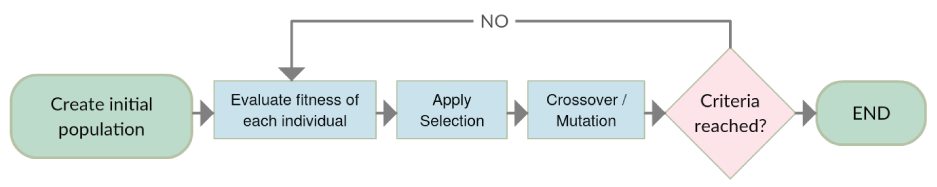
\includegraphics[width=310pt]{graphics/ga.png}
  \caption{Genetic Algorithm procedure}
  \label{fig:ga}
\end{figure}


The procedure for genetic algorithm can be described as follows, see Figure \ref{fig:ga}:

\begin{enumerate} 
\item \textit{Create initial population }– First an initial population is created, either on random or through some type of sampling (e.g. Latin hyper sampling \cite{10.2307/1268522}).
\item \textit{Evaluate fitness of each individual} – The objective function is called which gives each individual a score (heuristic).
\item \textit{Apply selection} – The individuals with a high fitness score have a higher chance to by selected for crossover, a biological metaphor for mating.
\item \textit{Crossover/Mutation} – The individuals with a high fitness recombine properties (in this context design variables) with each other, to create a new generation. Introducing a small chance of mutation, a random change, when two individuals crossover can minimize the risk of the algorithm to get trapped in local optima. Elitism can be introduced to always allow the best performing individuals to move to the next generation, which can improve convergence. 
\item \textit{End} – The procedure continues until a preselected criterion is reached, often number of generations or when solution stops to converge.
\end{enumerate} 


A weakness of genetic algorithm is that it can be very computationally heavy, as the objective function needs to be called for each new individual. There is also a lot of fine tuning, different types and rates of crossovers, mutations etc. 

A strength of the algorithm is that multiple well performing solutions can be presented fore the user (different individuals from the population). This can be used in conceptual design, where an aesthetically attractive well-performing solution is sought. The algorithm can also be used for interactive optimization \cite{Scott2002}, where a user can intervene the selection process to move the population in a desired direction. The algorithm has also been adjusted for use with multiple objective optimization, where the population converges to the Pareto front \cite{deb2002fast}.

\subsection{Topology optimization}
To optimize the material layout, given a set of boundary conditions and external forces, topology optimization can be used. The method can be implemented through the use of finite element analysis combined with optimization methods \cite{bendsoe2009topology}. However, the resulting optimal material layout can be infeasible to build due to high complexity.

\section{Eigenvalue analysis}
Eigenvalue analysis can be used to find the dynamic or static modal shapes for a structural model. From the stiffness matrix K of a structure, a set of scalar stiffness values can be determined \cite{Olsson2003}. Assume that a set of displacements a exists, that are proportional to a corresponding set of forces f, i.e.

\begin{equation*}
\mathbf{f} = \lambda \mathbf{a}
\end{equation*}

This can be combined with a linear elastic finite element formulation, i.e.

\begin{equation*}
\mathbf{Ka} =\mathbf{f} = \lambda \mathbf{a}
\end{equation*}

Which can be rewritten as

\begin{equation*}
(\mathbf{K} - \lambda \mathbf{I})\mathbf{a} = 0
\end{equation*}

This is a standard eigenproblem. The eigenvalues   $\lambda$ have the unit force/length, also called canonical stiffness values \cite{Olsson2006}. Every eigenvalue  $\lambda_i$ has a corresponding eigenvector   $\mathbf{a_i}$ , which describes a modal shape. Eigenvalues equal to zero means zero energy is required to form the corresponding modal shape, i.e. a rigid body motion. The eigenvectors are only defined within a scalar multiple. To create an animation of the modal shape, the eigenvector can be normalized and multiplied with a positive and negative scalar. This result in two different shapes, interpolation between the two shapes can then be used to create an animation.


\section{Graphic statics}
Graphic statics is a graphical method to find funicular shapes and compute forces for structural models through the use of a force diagram. The method was first published in 1886 by Karl Culmann \cite{Culmann1866}, the method was widely used until the 1970s, when the increase in computational power made numerical simulations widely available. 

The method has recently gained attention from the research community \cite{Todisco2015, Block, Fivet2013} because of its simplicity and power. However, the method is limited to statically determinate problems with axially loaded members. 
